% Options for packages loaded elsewhere
\PassOptionsToPackage{unicode}{hyperref}
\PassOptionsToPackage{hyphens}{url}
%
\documentclass[
]{article}
\usepackage{amsmath,amssymb}
\usepackage{lmodern}
\usepackage{iftex}
\ifPDFTeX
  \usepackage[T1]{fontenc}
  \usepackage[utf8]{inputenc}
  \usepackage{textcomp} % provide euro and other symbols
\else % if luatex or xetex
  \usepackage{unicode-math}
  \defaultfontfeatures{Scale=MatchLowercase}
  \defaultfontfeatures[\rmfamily]{Ligatures=TeX,Scale=1}
\fi
% Use upquote if available, for straight quotes in verbatim environments
\IfFileExists{upquote.sty}{\usepackage{upquote}}{}
\IfFileExists{microtype.sty}{% use microtype if available
  \usepackage[]{microtype}
  \UseMicrotypeSet[protrusion]{basicmath} % disable protrusion for tt fonts
}{}
\makeatletter
\@ifundefined{KOMAClassName}{% if non-KOMA class
  \IfFileExists{parskip.sty}{%
    \usepackage{parskip}
  }{% else
    \setlength{\parindent}{0pt}
    \setlength{\parskip}{6pt plus 2pt minus 1pt}}
}{% if KOMA class
  \KOMAoptions{parskip=half}}
\makeatother
\usepackage{xcolor}
\IfFileExists{xurl.sty}{\usepackage{xurl}}{} % add URL line breaks if available
\IfFileExists{bookmark.sty}{\usepackage{bookmark}}{\usepackage{hyperref}}
\hypersetup{
  pdftitle={Retaliation on a voodoo doll symbolizing an abusive supervisor restores justice},
  pdfauthor={Damien Dupré},
  hidelinks,
  pdfcreator={LaTeX via pandoc}}
\urlstyle{same} % disable monospaced font for URLs
\usepackage[margin=1in]{geometry}
\usepackage{graphicx}
\makeatletter
\def\maxwidth{\ifdim\Gin@nat@width>\linewidth\linewidth\else\Gin@nat@width\fi}
\def\maxheight{\ifdim\Gin@nat@height>\textheight\textheight\else\Gin@nat@height\fi}
\makeatother
% Scale images if necessary, so that they will not overflow the page
% margins by default, and it is still possible to overwrite the defaults
% using explicit options in \includegraphics[width, height, ...]{}
\setkeys{Gin}{width=\maxwidth,height=\maxheight,keepaspectratio}
% Set default figure placement to htbp
\makeatletter
\def\fps@figure{htbp}
\makeatother
\setlength{\emergencystretch}{3em} % prevent overfull lines
\providecommand{\tightlist}{%
  \setlength{\itemsep}{0pt}\setlength{\parskip}{0pt}}
\setcounter{secnumdepth}{-\maxdimen} % remove section numbering
\ifLuaTeX
  \usepackage{selnolig}  % disable illegal ligatures
\fi

\title{Retaliation on a voodoo doll symbolizing an abusive supervisor
restores justice}
\usepackage{etoolbox}
\makeatletter
\providecommand{\subtitle}[1]{% add subtitle to \maketitle
  \apptocmd{\@title}{\par {\large #1 \par}}{}{}
}
\makeatother
\subtitle{A model paper based on simulation data to explain the
principle of academic writing}
\author{Damien Dupré}
\date{}

\begin{document}
\maketitle

\hypertarget{abstract}{%
\subsection{Abstract}\label{abstract}}

The present paper draws from the paper entitled ``Righting a wrong:
Retaliation on a voodoo doll symbolizing an abusive supervisor restores
justice'' (Liang et al., 2018). This academic article was published in
the journal ``The Leadership Quarterly'' and has been awarded with the
prestigious IG Nobel Price (section Business Studies). The paper looked
at how subordinate retaliation moderates the relationship between
abusive supervision and subordinate injustice perception. More
precisely, the authors asked their participants to imagine an abusive or
non-abusive supervision context and they measured how much using a
virtual voodoo doll, representing the supervisor, would restore people's
sense of justice. By testing the hypotheses formulated by its authors on
simulated data, the present paper will describe each step of the
academic writing.

\hypertarget{introduction}{%
\section{Introduction}\label{introduction}}

Abusive supervision is a problem for the mental well-being of employees.
In cases of behaviours charactering abusive supervision such as such as
public ridicule, yelling, scapegoating, or other forms of supervisor
mistreatment, employees will have to deploy coping-mechanisms in order
to preserve enough motivation to work in this negative environment. The
premise of the paper Righting a wrong: Retaliation on a voodoo doll
symbolizing an abusive supervisor restores justice is that ``a natural
response for the subordinate is to directly retaliate against the
abusive supervisor'' (Liang et al., 2018, p.~443). This premise is
probably what made the paper published by Liang et al.~(2018) an
excellent candidate for the IG Nobel. However, this paper has an
excellent structure and a very robust method. For these reasons, it will
be used as example of how to write an academic paper.

The first step of an academic paper is the Introduction section which is
supposed 1) to present the problem that the paper is trying to
understand and 2) to end with the author's research question. Here the
research question of Liang et al.~(2018) can be summarised as the
following: How abusive supervision and subordinate retaliation influence
the subordinate injustice perception?

\hypertarget{literature-review}{%
\section{Literature Review}\label{literature-review}}

The literature review is used to describe each concept included in the
research question, independently, and in specific subsections. It aims
to give a short and up-to-date presentation of the current state of the
research involving these concepts with some example of results obtained
in this research. Here, there are three concepts to investigate: abusive
supervision, subordinate retaliation and subordinate injustice
perception.

\hypertarget{abusive-supervision}{%
\subsection{Abusive Supervision}\label{abusive-supervision}}

The goal of the present paper is to describe the process of academic
writing and not to investigate any kind of abusive supervision,
subordinate retaliation or subordinate injustice perception. This
subsection is only an example of structure.

\hypertarget{subordinate-retaliation}{%
\subsection{Subordinate Retaliation}\label{subordinate-retaliation}}

Sections in the literature review should present the state of the art of
previous scientific research investigating these variables and their
relationship. It is strongly recommended to use theories that have
already been published and to describe how they are relevant to you. You
can also use references from previous research to give some context to
the evidence that has been found. This scientific evidence should
support the formulation of your hypotheses.

\hypertarget{injustice-perception}{%
\subsection{Injustice Perception}\label{injustice-perception}}

The most important content of the literature review is the formulation
of hypotheses. These hypotheses can be implicitly formulated in the body
of the literature review but a common and efficient way to present the
hypotheses is explicitly at the end of the literature review.

\textbf{Hypothesis 1}: \emph{The average injustice perception in the
condition of abusive supervision is higher than the average injustice
perception in the condition of non-abusive supervision.}

\textbf{Hypothesis 2}: \emph{The injustice perception decrease when the
subordinate retaliation increase.}

\textbf{Hypothesis 3}: \emph{The effect of subordinate retaliation on
injustice perception in the condition of abusive supervision is higher
than in the condition of non-abusive supervision}

\hypertarget{method}{%
\section{Method}\label{method}}

The method section usually describes the participants/observations, the
material used to collect the data, the procedure followed by the authors
and the analyses performed.

\hypertarget{participantsobservations}{%
\subsection{Participants/Observations}\label{participantsobservations}}

In general, the participant section indicates the average age with
standard deviation, the number of male and female participants (and
other answers) and their origin. This selection also states how they
were recruited or selected. Here, 2000 participants are created
randomly.

\hypertarget{material}{%
\subsection{Material}\label{material}}

To manipulate abusive supervision, Liang et al.~(2018) have asked their
participants to imagine themselves in a condition of abusive supervision
or non-abusive supervision. Consequently, this variable is categorical
with two categories: abusive (N = 1015) and non-abusive (N = 985).

The method that Liang et al.~(2018) used to measure subordinate
retaliation is original and novel. They asked some of their participants
to use a virtual voodoo doll as if they were the subordinate imagining
that the doll was the abusive supervisor. Liang et al.~(2018) examined
whether participants used or not the virtual voodoo doll. However, for
the purposes of this paper, it is considered how long participants are
using the virtual voodoo doll (measured in seconds). As a result the
variable is continuous which explains how Hypothesis 2 is formulated.

Liang et al.~(2018) used a word completion task to measure subordinate
injustice perception. In this task, five words have missing letters, and
have to be completed so that they become either a neutral word or a
negative word. The ratio of negative words used among the five words is
supposed to reveal the injustice perception still felt by the
subordinate. The measurement of subordinate injustice perception is
simulated to have the same shape as the data obtained from this task.

\hypertarget{procedure}{%
\subsection{Procedure}\label{procedure}}

As indicated previously, the data are simulated.

\hypertarget{data-analysis}{%
\subsection{Data Analysis}\label{data-analysis}}

Here comes the main part of the method section. The absence of a Data
Analysis section in an academic paper reveals its poor quality. However,
by including both the graphic representation of the model tested and its
corresponding equation, authors can display the robustness of their
analyses.

The model is represented Figure 1 where AS is abusive supervision, IP is
injustice perception, and SR is subordinate retaliation. It shows a
classic moderation model which is the alternative name for interaction
effect. A note of caution; a default moderation model includes not only
the interaction-effect hypothesis but also the main effect hypotheses of
the two predictors which is not obvious from the model representation.

\begin{figure}
\centering
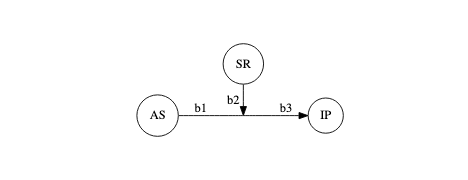
\includegraphics{voodoo_report_final_files/figure-latex/unnamed-chunk-1-1.png}
\caption{Representation of the model testing the three hypotheses (AS =
abusive supervision; IP = injustice perception; SR = subordinate
retaliation).}
\end{figure}

In a model each arrow is an hypothesis, also represented by the symbol
\(b\). The test of all hypotheses in the same model will be done by
analysing the following equation:

\[ IP = b_0 + b_1 AS + b_2 SR + b_3 AS * SR + e \]

In the slides presented earlier, the general linear regression model was
presented as the unique solution to test any hypothesis with any kind of
variable. The use of t-tests or ANOVA is correct but they are special
cases of the linear regression models. This multiple linear regression
could be tested in any statistical software but I would strongly
recommend jamovi (The jamovi project, 2021).

\hypertarget{results}{%
\section{Results}\label{results}}

The results section does not have to be long; it only needs to include
some information about the variables, mainly their mean and standard
deviation. This information can also include validity or reliability
measures if not presented in the method section. Here, the average time
spent using the virtual voodoo doll was 100s (SD = 20s), the shortest
time spent was 28s and the longest 167s. However, 100 values are missing
from the subordinate retaliation variable (voluntarily removed). The
average proportion of negative words (from the word completion task) is
49.9\% (SD = 28\%).

Next, is the inferential statistics information, which has two parts:
description of the overall model accuracy and test of each hypothesis.
First, the model including both main effects of abusive supervision and
subordinate retaliation as well as their interaction effect explains a
significant part of subordinate injustice perception (R\^{}2 = 0.498,
F(3,1896) = 626, p \textless{} 0.001). More precisely, the model
explains 49.8\% of the variance of injustice perception.

To interpret the statistics behind hypothesis testing, only the p-value
is necessary. A p-value higher than indicates that the null hypothesis
is true whereas a p-value lower than 0.05 indicates that the null
hypothesis is rejected, and the alternative hypothesis considered as
plausible. In the current simulated data, the results reveal a
significant effect of abusive supervision on injustice perception (b =
-0.09956, 95\%CI{[}-0.19535,-0.00378{]}, t(1896) = -2.039, p = 0.042).
This means that being in a non-abusive supervision context decreases, on
average, by 9.95\% the amount of negative words in the completion task.
They also reveal a significant effect of subordinate retaliation on
injustice perception (b = -0.00858, 95\%CI{[}-0.00925,-0.00790{]},
t(1896) = -24.969, p \textless{} 0.001). More precisely, for every
second spent with the virtual voodoo doll, the amount of negative words
in the completion task decreases by 0.8\%. Finally the results did not
reveal a significant interaction effect (or moderation effect) between
abusive supervision and subordinate retaliation on injustice perception
(b = -0.000213, 95\%CI{[}-0.00115,0.000724{]}, t(1896) = -0.445, p =
0.656) as show in Figure 2.

\begin{figure}
\centering
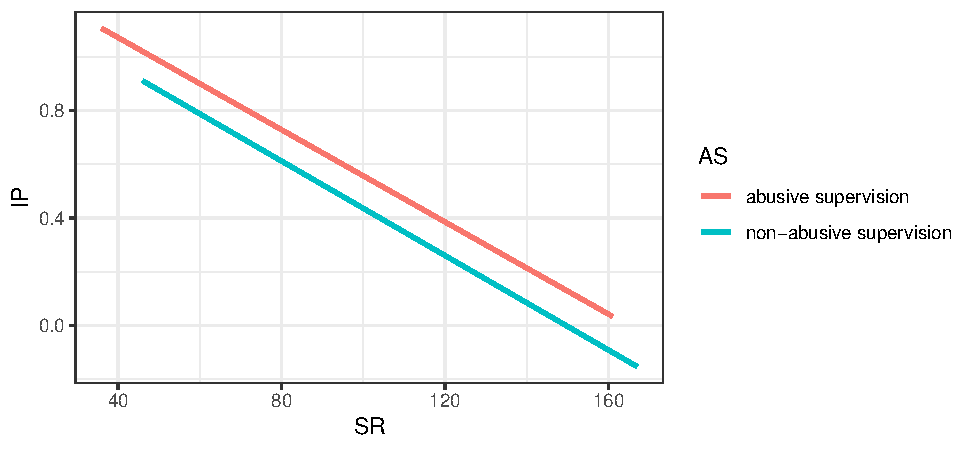
\includegraphics{voodoo_report_final_files/figure-latex/unnamed-chunk-2-1.pdf}
\caption{The slope of the relationship between subordinate retaliation
and injustice perception is not different for abusive supervision and
non-abusive supervision contexts (AS = abusive supervision; IP =
injustice perception; SR = subordinate retaliation).}
\end{figure}

\hypertarget{discussion-and-conclusion}{%
\section{Discussion and Conclusion}\label{discussion-and-conclusion}}

The purpose of the current paper was to display the structure of a
research paper rather than actually writing a paper. In this section,
authors are presenting potential explanations for the effect/non-effect
obtained. Limitations regarding the data collection and data analyses
can also been added in these sections. Here, the data were randomly
generated. Your task is to conduct your own discussion based on the
results you obtain and the hypotheses which you formulate.

\hypertarget{references}{%
\section{References}\label{references}}

Liang, L. H., Brown, D. J., Lian, H., Hanig, S., Ferris, D. L., \&
Keeping, L. M. (2018). Righting a wrong: Retaliation on a voodoo doll
symbolizing an abusive supervisor restores justice. The Leadership
Quarterly, 29(4), 443-456.

The jamovi project (2021). jamovi (Version 1.6). Retrieved from
\url{https://www.jamovi.org}.

\end{document}
